
\documentclass[letterpaper,twocolumn,10pt]{article}
\usepackage{usenix,epsfig,endnotes}
\usepackage{graphicx}
\usepackage{subfigure}

\setlength{\parskip}{0pt plus 1pt minus 1pt}
%\setlength{\parsep}{0pt plus 1pt minus 1pt}
\setlength{\parsep}{0pt}
%\setlength{\partopsep}{} 
%    \topsep 

%%%reduce the margin places between floats including pictures and tables and text
\setlength{\floatsep}{0in}
\setlength{\textfloatsep}{3pt plus 1.0pt minus 2.0pt}
\setlength{\intextsep}{3pt plus 1.0pt minus 2.0pt}
\setlength{\dbltextfloatsep}{3pt plus 1.0pt minus 2.0pt}
\setlength{\dblfloatsep}{3pt plus 1.0pt minus 2.0pt}
\setlength{\abovecaptionskip}{1pt plus 1.0pt minus 1.0pt}
\setlength{\belowcaptionskip}{2pt plus 1.0pt minus 1.0pt}

\graphicspath{{figs/}}
\begin{document}

%don't want date printed
\date{}

%make title bold and 14 pt font (Latex default is non-bold, 16 pt)
\title{\Large \bf Fast Logging and Recovery on Single Node with Multi-core}

%for single author (just remove % characters)
\author{
{\rm Youhui Bai}\\
USTC\\
youhuibai0108@gmail.com
\and
{\rm Cheng Li}\\
USTC\\
chenglinkcs@gmail.com
% copy the following lines to add more authors
\and
{\rm Yinlong Xu}\\
USTC\\
ylxu@ustc.edu.cn
}
 % end author

\maketitle

% Use the following at camera-ready time to suppress page numbers.
% Comment it out when you first submit the paper for review.
\thispagestyle{empty}
% \section{Background and Related Work}

Previous works focus on mining relationships among files according to their access pattern. If two files are frequent accessed closely in the past, they will be accessed together with higher probability near the future. Based on this definition, C-Miner\cite{li2004c} adopts a frequent sequence mining method to explore block correlations. DiskSeen\cite{ding2007diskseen} exploits disk layout and based on analysis tof temporal and spatial relationships to improve the sequentiality of disk access. 

To reduce the IOs to file system, Kroeger\cite{kroeger2001design} introduces a extended partitioned context modeling(EPCM) to explore correlations by building access trie according to access pattern and prefetches the files with the highest weight. Gu\cite{gu2010novel} proposes a the weighted-graph-based grouping method to predict and prefetch the following access sequence.

These above two methods require extra space to store the correlations and the algorithm complexity is heavy. Meanwhile, based on the access pattern to exploring correlations is offline, but the correlations among files will evolve as time goes. And they only consider the access pattern and forget the intrinsic relations among files. 

\section{Background and Motivations}
Failures(e.g., process crash, kernel panics, power outages) are common in systems like Database systems and File systems, even in robust enough Distributed systems, which will incur fatal problems such as inconsistency and data loss. Techniques have been proposed to address these issues, for example, systems offten leverage Log and Replication to handle failures. In this paper, we focus on Log especially write-ahead log, systems will log changes into Log for persistency, then to the real place,  When restarting, systems recovery from Log take advantage of full operation informations in Log.

But the logging when forward processing and recovery from Log after failures are both too slow to support high-level application well, which is intolerable even for a single node. the architeture and process flow of a single node is illustrated as Fig.~\ref{fig:architecture}. The \texttt{Disk} and \texttt{Dram} are managed by page. When transactions want to operate, they map the operations into Data buffer in step 1, then log the operations in Log buffer in step 2, the log entries in Log buffer will be flushed to durable storage for persistency in step 3, then, if the flush returns successfully in step 4, the system will inform user that the operations are completed, and the system will flush the dirty page in Data buffer into durable storage later in step 5.

Generally, systems leverage single Log to log and recover for simple, this is why the logging and revovery are so slow. First, the multiple threads will contend to write to a single Log, second, a sequential scan will be performed over the corresponding log by only one thread. Both of them will cause worse scalability as the number of threads grows in a single node with multi-core.

A straightforward approach to speed up the logging and recovery is distributing the Log, for example, one Log file per processor. But the distributed Log is still tardy because of too many cross-log dependencies.

In this paper, we propose a new version of distributed Log by leveraging a few techniques, which will support parallelism well in single node with multi-core.
% Modern distributed file systems, such as GFS\cite{ghemawat2003google}, HDFS\cite{shvachko2010hadoop}, Ceph\cite{weil2006ceph}, which consist of three components, metadata servers(MDS), object-based storage devices(OSD) and clients as Fig.~\ref{fig:architecture} shows. Clients perform metadata operations(\emph{open, stat}) directly with MDS and file I/O directly with data server. This architecture decouples metadata I/O from data IO and increases overall scalability. For example, client requests data with pathname /var/log/client.log. By multiple interactions to MDS, client lookups the directory of \texttt{root}, \texttt{var} and \texttt{log} to locate the inode of \texttt{client.log} and checks the permission. Once client obtain the inode, it must get the capability to access to data. Then, client will request a lease on this file to MDS. Finnaly, client interact with OSD to operator file I/O. Due to the iterative lookup and checking permission operations, the IOs between clients and MDS are more than OSD. Because overall 50\% of IOs are to metadata\cite{roselli2000comparison}, metadata performance is crucial.

% \begin{figure}[htbp]
%   \centering
%   % Requires \usepackage{graphicx}
%   %\vspace{-5pt}
%   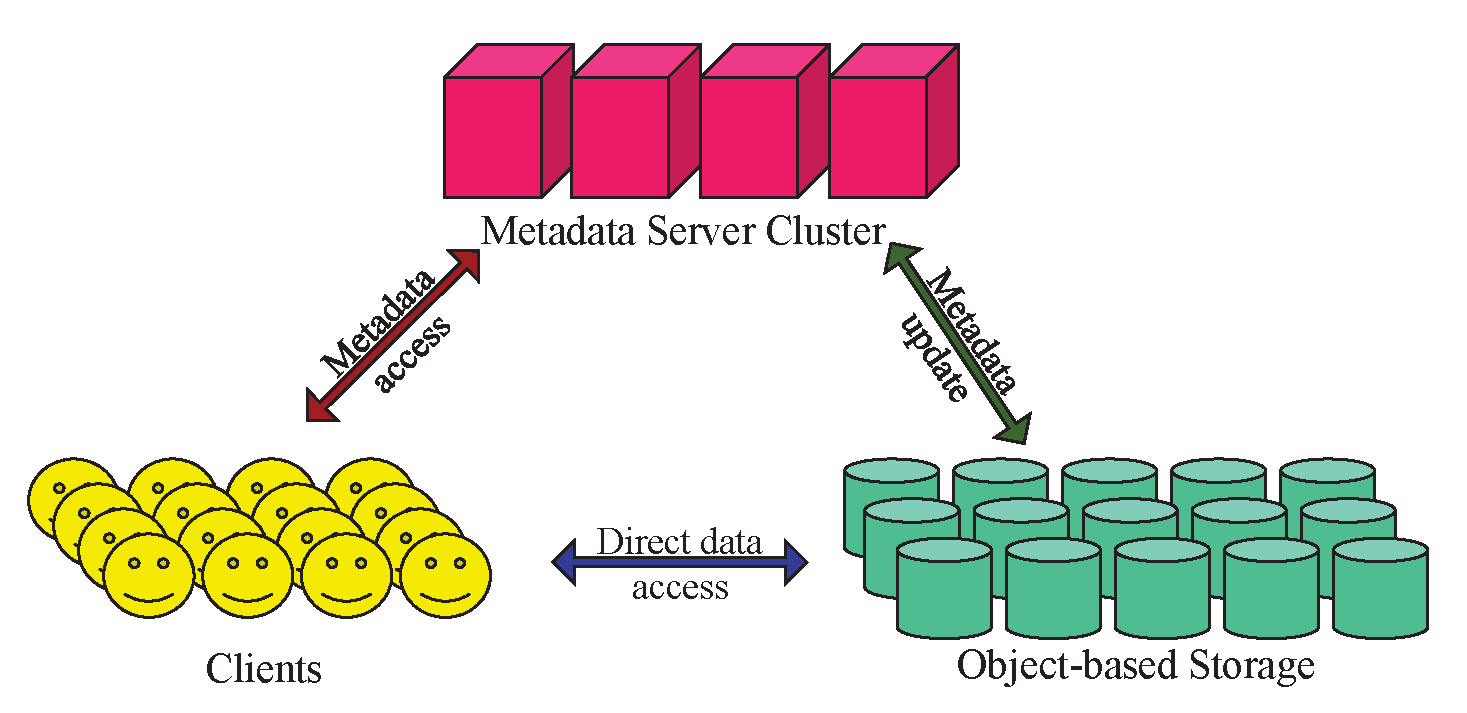
\includegraphics[width=1\linewidth]{architecture.eps}\\
%   %\vspace{-10pt}
%   \caption{Architecture of distributed file systems.}\label{fig:architecture}
%    %\vspace{-10pt}
% \end{figure}
\begin{figure}[htbp]
  \centering
  % Requires \usepackage{graphicx}
  %\vspace{-5pt}
  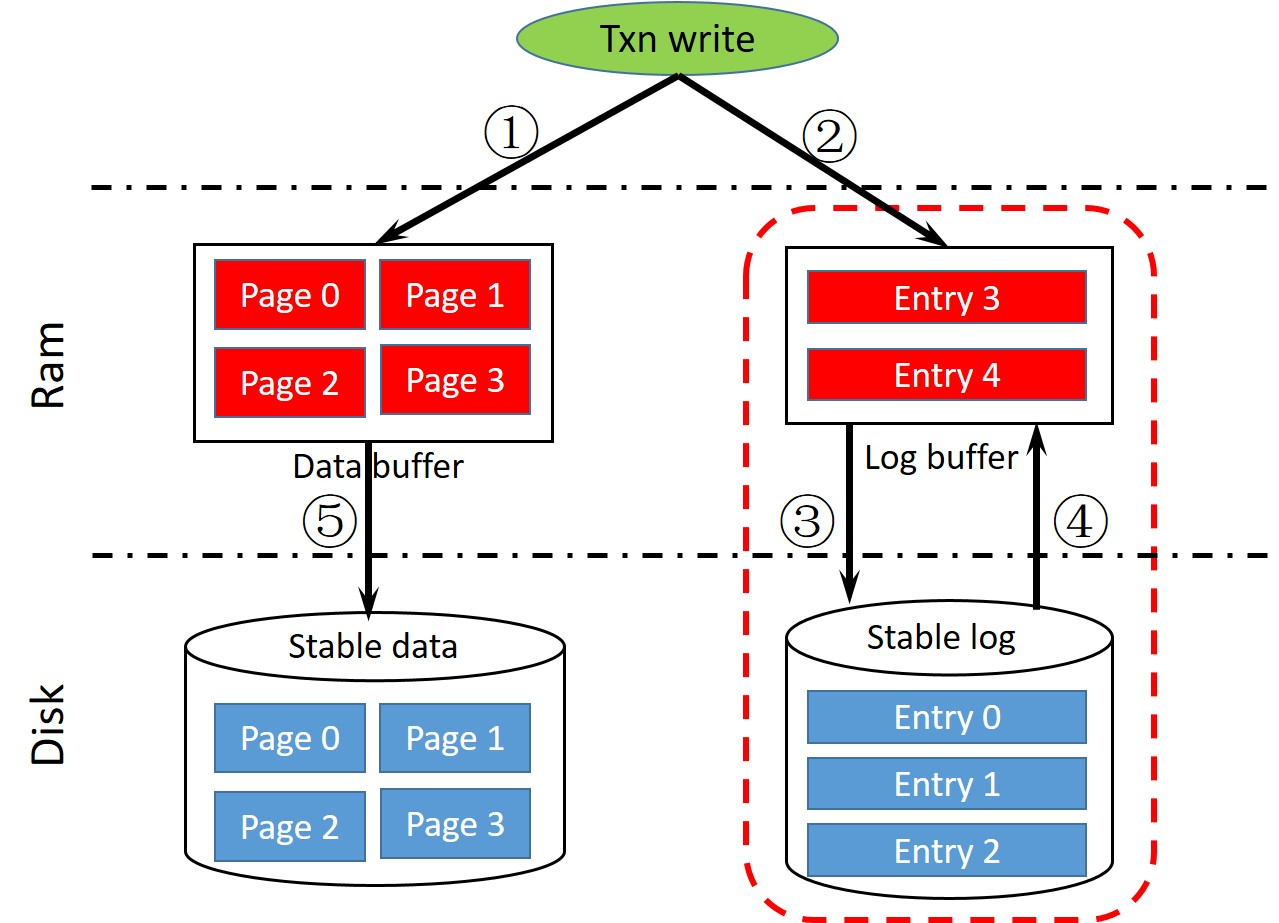
\includegraphics[width=1\linewidth]{architecture.jpg}\\
  %\vspace{-10pt}
  \caption{Architecture and process flow of write-ahead logging.}\label{fig:architecture}
   %\vspace{-10pt}
\end{figure}


% In this paper, we propose a correlations-based metadata prefetching to reduce IO traffic to MDS, to scale distributed file systems, to increase client cache hit ratio with high accuracy and low false positive. How to define the correlations among files and how to update correlations in real time become a challenge.


\section{Our Approach and Novelty}
\subsection{Correlations Definition}

We think that file A and file B are correlated if file A refers to file B or they are accessed closely. In our model, there are two types of correlations which are data correlation and access correlation respectively. If a file refers or links to another file, for example web file contains the links to scripts, images or other links, these two files are data related. And if two files often access closely, these two files are access related.

Both in data correlation or access correlation, the correlations between files are different. For example, scripts and images are more related than links in web files because the links maybe not clicked by clients but the scripts and images must be loaded when the web files load. Therefore, we introduce a priority to stands for the closer correlations in file system.
\begin{figure}[htbp]
  \centering
  % Requires \usepackage{graphicx}
  %\vspace{-5pt}
  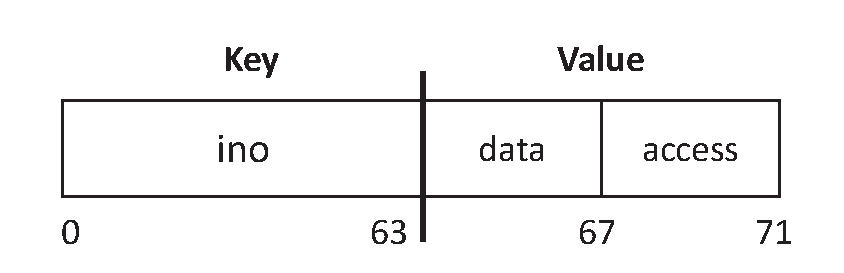
\includegraphics[width=0.8\linewidth]{data_structure.eps}\\
  %\vspace{-10pt}
  \caption{Data structure of correlation.}\label{fig:data-structure}
   %\vspace{-10pt}
\end{figure}

We propose a key-value structure for correlations as Fig.~\ref{fig:data-structure} shows. The Key is the inode number of the correlated file and occupies 8 Bytes. To keep uniqueness of key, inode number should be always increasing. The value is the score of two correlations to make a priority between correlations. The closer correlations are with higher scores.

\subsection{Correlations Update}

In order to give a better presentation to correlations, we propose three update methods which are online update, offline update and user interface as Fig.~\ref{fig:design} shows.
\begin{figure}[htbp]
  \centering
  % Requires \usepackage{graphicx}
  %\vspace{-5pt}
  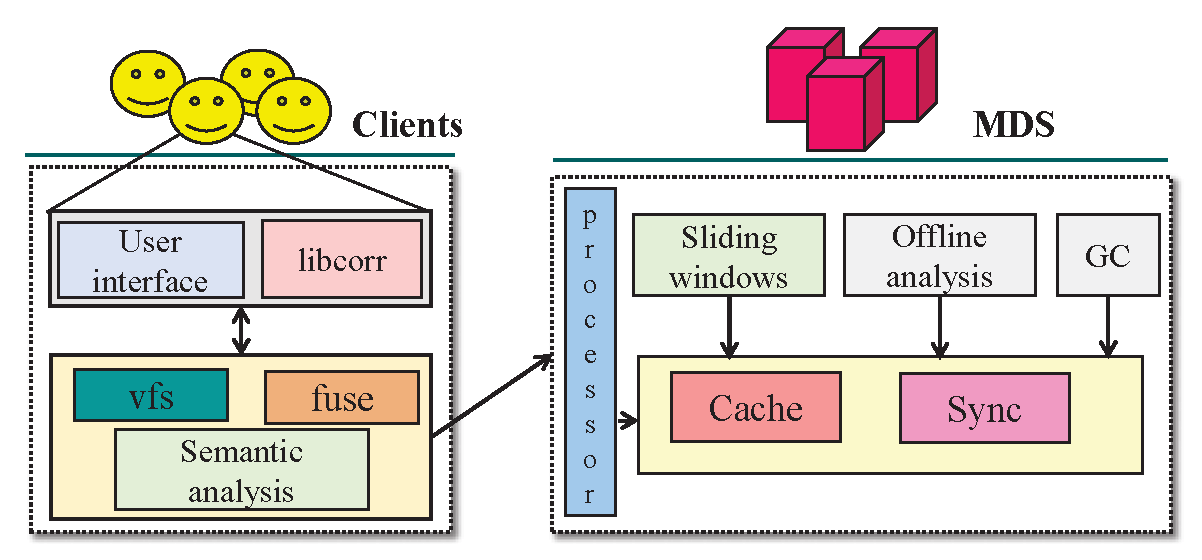
\includegraphics[width=1\linewidth]{design2.eps}\\
  %\vspace{-10pt}
  \caption{Correlations update.}\label{fig:design}
   %\vspace{-10pt}
\end{figure}

\textbf{Online update} Semantic analysis and sliding windows procedures are responsible for updating correlations online. When clients update files data, semantic analysis procedure will be trigged to update data correlations in real time. Due to the diverse data formats with multiple types of files, the design of semantic analysis procedure becomes a challenge. For example, scripts, images or other files are linked in web file by \texttt{href} or \texttt{src}. And source code file includes head file by \texttt{include}. Based on the diverse data organization, we propose a aggravate semantic analysis proceeding to file data.

We build a semantic set for different types of files. Each element is responsible for a specific type. When new data is written, the analysis process is triggered. Based on the matching patterns that we pre-defined, this process scans the data to explore the related files and records them. Each correlation is scored by files types and counted to make a difference of correlations.

We create a sliding window on recently access pattern of every client to exploring online access correlations and to exclude concurrency interference simultaneously. The window is with a fixed size and slides ahead as new access sequence comes. The files in window are considered correlated and recorded as \emph{ordered pairs} to keep their access sequence. Each ordered pair has a count and alters dynamically with window slides. Meanwhile, the correlation is higher when access to two files is closer. Hence count and gap are both considered into score.

\textbf{Offline update} Consider that the quality of service, online exploring must be lightweight. To give a better presentation to correlations, we propose a offline method to exploring correlations among files when the system is idle or light-loaded. System will record the access pattern for every client in past which is longer than the online windows and build a access trace to be analysed. To find the correlations among such access traces, a machine learning or deep learning will be adopted. The results are updated in files extended attributes. With offline exploring, more correlations could be found which is not only in single client, but also between clients.

\textbf{User interface} Besides semantic analysis and sliding windows, we also support multiple user interfaces for clients update. All interfaces are supported POSIX interface and need not change clients applications.
\begin{itemize}
  \item \textbf{Set} Clients could set data and access correlations to a specific file with this interface. New score will be embedded into system.
  \item \textbf{Remove} Remove a specific correlation item from a file.
\end{itemize}

Besides set and remove interfaces, we also support clients \textbf{get} a specific correlation from a file or \textbf{list} all correlations together.

\textbf{Challenge 1} When there is overwritten to a file, as Fig.~\ref{fig:overwrite} shows, the new data is easy to make a analysis to find correlated files. But the overlayed data maybe contain links to related files, which are obsolete and should be removed simultaneously. However the covered data isn't in cache, so how to update the correlations is a challenge. We introduce a lazy update method. When a files overwrites, we make a \texttt{overwritten} tag on the file. Once the tagged file is accessed, system will make a semantic analysis again to rebuild correlations to keep consistency.
\begin{figure}[htbp]
  \centering
  % Requires \usepackage{graphicx}
  %\vspace{-5pt}
  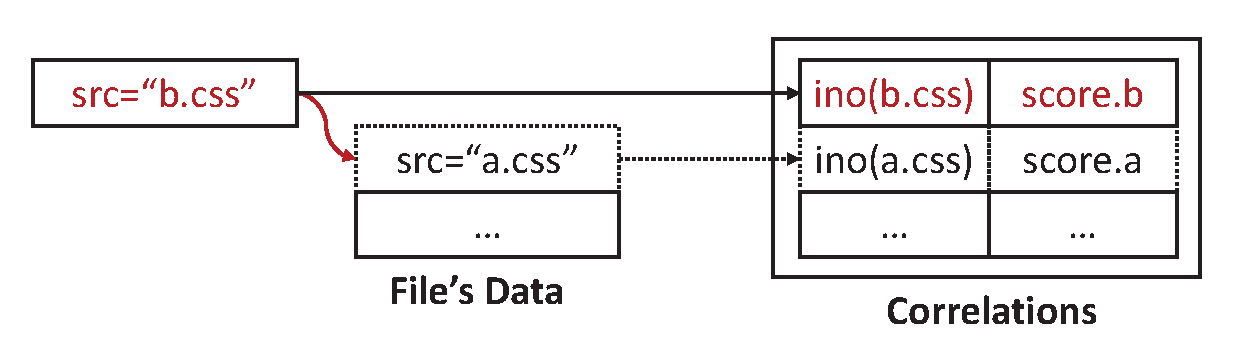
\includegraphics[width=1\linewidth]{overwrite.eps}\\
  \vspace{-10pt}
  \caption{Lazy update for obsolete correlations when deleting files.}\label{fig:overwrite}
   %\vspace{-10pt}
\end{figure}

\textbf{Challenge 2} When a file is deleted, the correlations to it which contained in other files becomes obsolete and should be removed at the same time. As Fig.~\ref{fig:remove} depicts, file \texttt{a} is deleted. Other four files store a correlations to \texttt{a}. But the correlation is one-direct, system can't remove other correlations to file \texttt{a} right now. To reduce the operation's complexity and overhead, we reserve the obsolete correlations in origin inode. When the file is accessed, the obsolete correlations maybe fetched. Then at that time, these obsolete correlations are found and removed from inode.
\begin{figure}[htbp]
  \centering
  % Requires \usepackage{graphicx}
  %\vspace{-5pt}
  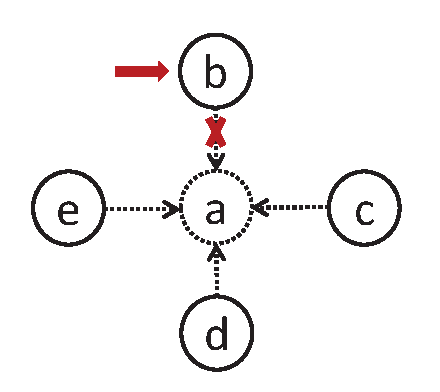
\includegraphics[width=0.5\linewidth]{remove.eps}\\
  %\vspace{-10pt}
  \caption{Lazy update for obsolete correlations when deleting files.}\label{fig:remove}
   %\vspace{-10pt}
\end{figure}

\subsection{Metadata Prefetching}

We propose a aggressive metadata prefetching method to reduce traffic to MDS. In order to increase the hit ratio and reduce space overhead in client, we restrict the number of prefetching items by setting a threshold of correlations scores. When the score of a correlation is higher than the threshold, we think that the correlation is closer and should be fetched together.

To reduce the lookup operations of directory across the network to check the permission, we also batch the ancestors information(directory and inode) with prefetching. System gives the same lease to correlated files as requested file due to the closer correlations. Once clients receive the batched metadata, they insert them into cache to service following requests.

\subsection{Implementation and Evaluation}

We are building a prototype system based on Ceph, which consists of 32 OSDs and one MDS cluster. We track the IO flows from client to MDS and embed online and offline exploring module into clients and MDS respectively. We are also creating a general library to support user interfaces which could be used for other file systems. We look forward to reducing IOs traffic and memory overhead to MDS and increasing client cache hit ratio via correlations-based metadata prefetching.





\section{Conclusion and Future Work}

In this paper, we give a presentation of correlations among files from the views of files data and access pattern. We define the correlations and support three methods to update them via online, offline and client-defined. Based on these correlations, we propose a approach to prefetch related metadata to reduce IOs traffic to MDS and increase client cache hit ratio. And we are building a prototype system to evaluate performance.

In the future, we are plan to conduct diverse experiments to compare our approach with other methods on IOs to MDS, client cache hit ratio and memory overhead. Meanwhile, we expect exploring correlations from other views, like clients and namespace to present a extensive view to correlations. 

\begin{footnotesize}
%\bibliographystyle{plain}
\bibliographystyle{abbrv}
\bibliography{paper}
\end{footnotesize}


\end{document}






